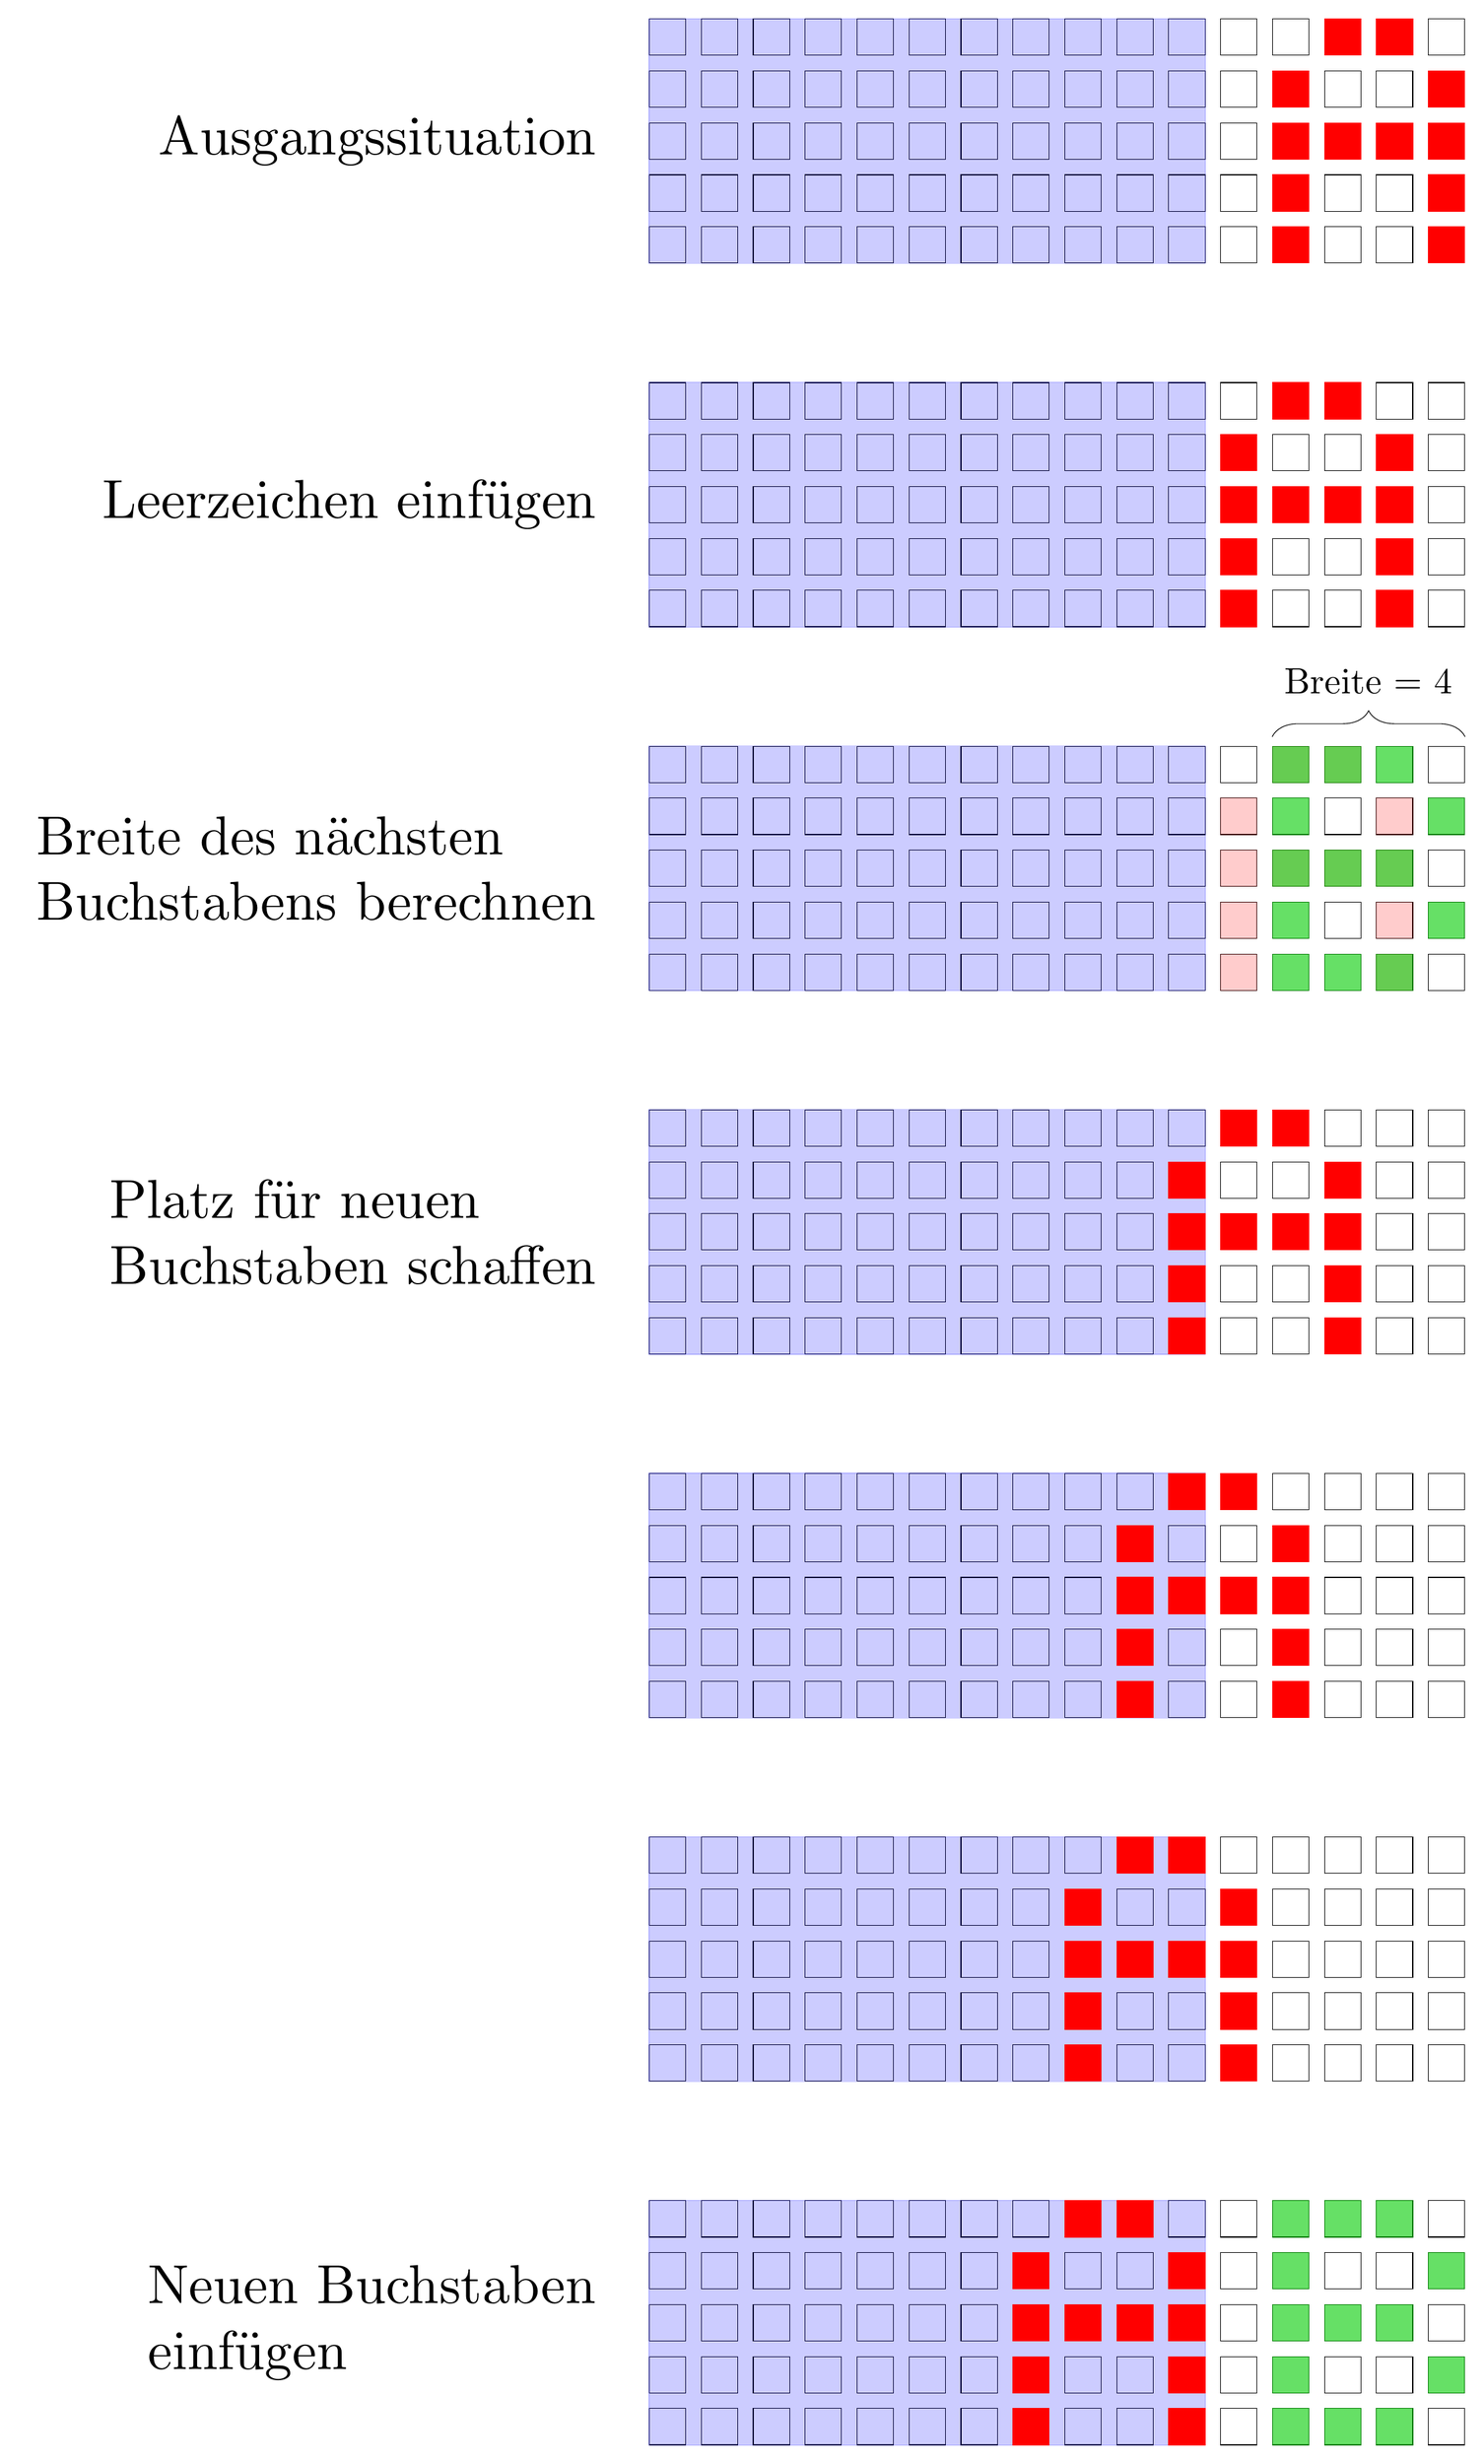
\begin{tikzpicture}[
	description/.style = { scale= 3 , align = left}
]
	\begin{scope}[yshift = 7cm]
		\foreach \x in {0,...,15}{
			\foreach \y in {0,...,4}
				\node [rectangle ,draw, inner sep=3.5mm](\x\y) at (\x,\y){} ;
		}
		\filldraw[blue, opacity=0.2] (00.south west) rectangle  (104.north east);
		\foreach \name in {120,121,122,123,132,134,142,144,150,151,152,153}
 		\fill [red](\name.south west) rectangle (\name.north east);

		\node [left, description] at (-1,2){Ausgangssituation};

	\end{scope}
% ----------------------------------------------
	\begin{scope}[yshift=0cm]
	\foreach \x in {0,...,15}{
			\foreach \y in {0,...,4}
				\node [rectangle ,draw, inner sep=3.5mm](\x\y) at (\x,\y){} ;
		}
		\filldraw[blue, opacity=0.2] (00.south west) rectangle  (104.north east);
		\foreach \name in {110,111,112,113,122,124,132,134,140,141,142,143}
 		\fill [red](\name.south west) rectangle (\name.north east);

		\node [left, description] at (-1,2){Leerzeichen einf$\ddot{\mathrm{u}}$gen};
		\end{scope}
% -----------------------------------------------
\begin{scope}[yshift=-7cm]
		\foreach \x in {0,...,15}{
			\foreach \y in {0,...,4}
				\node [rectangle ,draw, inner sep=3.5mm](\x\y) at (\x,\y){} ;
		}
		\filldraw[blue, opacity=0.2] (00.south west) rectangle  (104.north east);
		\foreach \name in {110,111,112,113,122,124,132,134,140,141,142,143}
 		\fill [red, opacity=0.2](\name.south west) rectangle (\name.north east);
		\foreach \name in {120,121,122,123,124,130,132,134,140,142,144,151,153}
 		\fill [green!80!black, opacity=0.6](\name.south west) rectangle (\name.north east);

		\node [left, description] at (-1,2){Breite des n$\ddot{\mathrm{a}}$chsten\\ Buchstabens berechnen};

		\draw [decorate, decoration = {brace, raise = 5pt, amplitude = 5mm}](124.north west) to node[above = 7.5 mm, scale = 2]{Breite = 4} (154.north east);
	\end{scope}
% ----------------------------------------------
	\begin{scope}[yshift=2*-7cm]
	\foreach \x in {0,...,15}{
			\foreach \y in {0,...,4}
				\node [rectangle ,draw, inner sep=3.5mm](\x\y) at (\x,\y){} ;
		}

		\filldraw[blue, opacity=0.2] (00.south west) rectangle  (104.north east);
		\foreach \name in {100,101,102,103,
										112,114,
										122,124,
										130,131,132,133}
 		\fill [red](\name.south west) rectangle (\name.north east);

		\node [left, description] at (-1,2){Platz f$\ddot{\mathrm{u}}$r neuen \\Buchstaben schaffen};
		\end{scope}
% ----------------------------------------------
	\begin{scope}[yshift=3*-7cm]
	\foreach \x in {0,...,15}{
			\foreach \y in {0,...,4}
				\node [rectangle ,draw, inner sep=3.5mm](\x\y) at (\x,\y){} ;
		}

		\filldraw[blue, opacity=0.2] (00.south west) rectangle  (104.north east);
		\foreach \name in {90,91,92,93,
										102,104,
										112,114,
										120,121,122,123}
 		\fill [red](\name.south west) rectangle (\name.north east);
		\end{scope}
% ----------------------------------------------
	\begin{scope}[yshift=4*-7cm]
	\foreach \x in {0,...,15}{
			\foreach \y in {0,...,4}
				\node [rectangle ,draw, inner sep=3.5mm](\x\y) at (\x,\y){} ;
		}

		\filldraw[blue, opacity=0.2] (00.south west) rectangle  (104.north east);
		\foreach \name in {80,81,82,83,
										92,94,
										102,104,
										110,111,112,113}
 		\fill [red](\name.south west) rectangle (\name.north east);
		\end{scope}

% ----------------------------------------------
	\begin{scope}[yshift=5*-7cm]
	\foreach \x in {0,...,15}{
			\foreach \y in {0,...,4}
				\node [rectangle ,draw, inner sep=3.5mm](\x\y) at (\x,\y){} ;
		}

		\filldraw[blue, opacity=0.2] (00.south west) rectangle  (104.north east);
		\foreach \name in {70,71,72,73,
										82,84,
										92,94,
										100,101,102,103}
 		\fill [red](\name.south west) rectangle (\name.north east);

		\foreach \name in {120,121,122,123,124,130,132,134,140,142,144,151,153}
 		\fill [green!80!black, opacity=0.6](\name.south west) rectangle (\name.north east);

		\node [left, description] at (-1,2){Neuen Buchstaben \\einf$\ddot{\mathrm{u}}$gen};
		\end{scope}

\end{tikzpicture}